\documentclass[11pt]{article}
\title{\textbf{Smart Classroom: System Architecture Overview}}
\author{Anou Oussama - El Hazal Salma - Lakhiri Rim}
\date{December 1, 2023}
\usepackage{fullpage}
\usepackage{graphicx}

\begin{document}
	\maketitle
	
	\section{System Block Definition Diagram}
	The system's Block Definition Diagram of the smart classroom project is illustrated in Figure \ref{fig:system-bdd}.
	
	\begin{figure}[h]
		\centering
		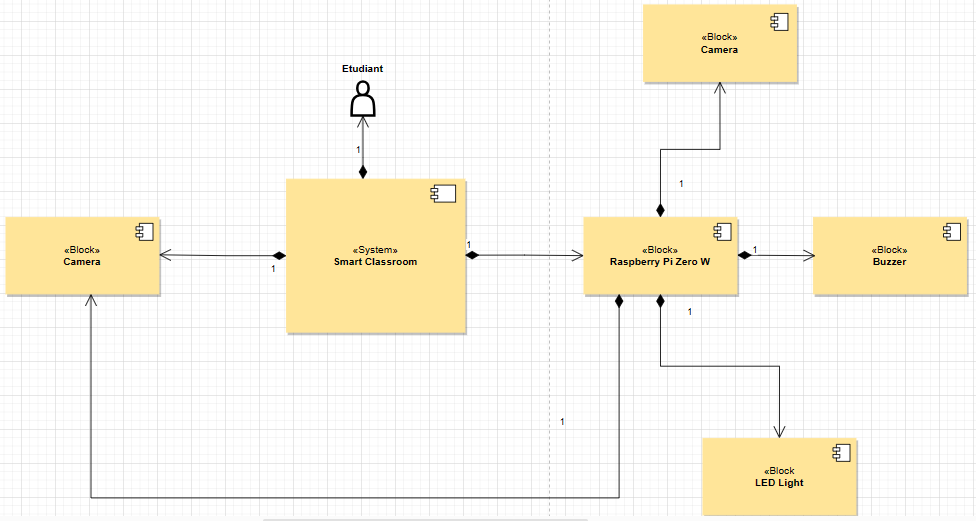
\includegraphics[width=0.7\textwidth]{SC.png}
		\caption{System Block Definition Diagram}\label{fig:system-bdd}
	\end{figure}
	
	\begin{itemize}
		\item \textbf{Camera:} Installed on the ceiling of the classroom, it records and saves the session.
		\item \textbf{Raspberry Pi:} Installed on the door frame and connected to a camera for capturing faces and performing facial recognition.
		\item \textbf{Buzzer:} Connected to the Raspberry Pi; emits sound in case of errors, such as failed facial recognition, with different sounds for successful recognition.
		\item \textbf{LED:} Connected to the Raspberry Pi; indicates successful or unsuccessful facial recognition through red or green lights.
	\end{itemize}
	
	\pagebreak
	
	\section{Raspberry Pi Block Definition Diagram}
	To provide more details, a Block Definition Diagram for the Raspberry Pi is presented in Figure \ref{fig:rpi-bdd}.
	
	\begin{figure}[h]
		\centering
		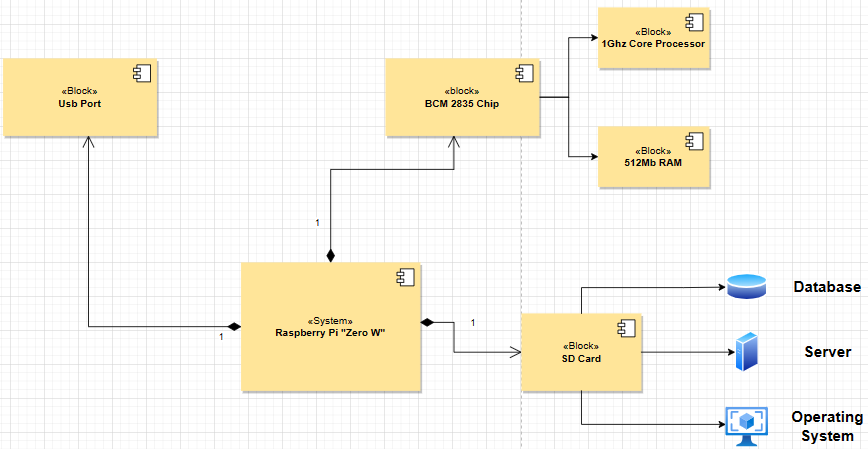
\includegraphics[width=0.7\textwidth]{RPi.png}
		\caption{Raspberry Pi Block Definition Diagram}\label{fig:rpi-bdd}
	\end{figure}
	
	\begin{itemize}
		\item \textbf{USB port:} Allows connection to a computer for programming the Raspberry Pi.
		\item \textbf{Core processor:} Serves as the central processing unit (CPU), executing instructions and performing calculations.
		\item \textbf{RAM:} Random Access Memory provides temporary storage for actively used or imminently needed data.
		\item \textbf{BCP chip:} Broadcom BCM283x series SoC processor; integrates essential components for the Raspberry Pi.
		\item \textbf{SD card:} Primary storage medium for the Raspberry Pi, storing the OS, software, user data, and necessary files.
	\end{itemize}
\end{document}
